\newpage\setcounter{dang}{0}
\section{VỊ TRÍ TƯƠNG ĐỐI CỦA HAI ĐƯỜNG THẲNG. GÓC \& KHOẢNG CÁCH}
\subsection{Tóm tắt lý thuyết}
\subsubsection{Vị trí tương đối giữa hai đường thẳng}
Mỗi đường thẳng trong mặt phẳng toạ độ là tập hợp những điểm có toạ độ thoả mãn phương trình của đường thẳng đó. Vì vậy, bài toán tìm giao điểm của hai đường thẳng được quy về bài toán giải hệ gồm hai phương trình tương ứng.\\
Trên mặt phẳng toạ độ, xét hai đường thẳng
$\Delta_1\colon a_1x+b_1y+c_1=0$ và $\Delta_2\colon a_2 x+b_2 y+c_2=0$.\\
Khi đó, toạ độ giao điểm của $\Delta_1$ và $\Delta_2$ là nghiệm của hệ phương trình
$$
\heva{&
	a_1x+b_1y+c_1=0 \\&
	a_2x+b_2y+c_2=0.}$$
\begin{note}
	\begin{itemize}
		\item $\Delta_1$ cắt $\Delta_2$ tại $M(x_0;y_0) \Leftrightarrow$ hệ $(*)$ có nghiệm duy nhất $(x_0; y_0)$.
		\item $\Delta_1$ song song với $\Delta_2 \Leftrightarrow$ hệ $(*)$ vô nghiệm.
		\item $\Delta_1$ trùng $\Delta_2\Leftrightarrow$ hệ $(*)$ có vô số nghiệm.	
	\end{itemize}
\end{note}
{\bf Chú ý}
\begin{center}
	\begin{tikzpicture}[line cap=round,line join=round,font=\footnotesize,scale=.7,>=stealth,thick]
		\draw (0,0) node (A)[below] {$\Delta_1$}--(7.5,0.5) node (B){};
		\draw (0,-2.5) node (C)[below] {$\Delta_2$}--(7.5,-2) node (D){};
		\path (5,-0.5) coordinate (E) (6,-1.5) coordinate (F);
		\coordinate (H) at ($(A)!(E)!(B)$);
		\coordinate (K) at ($(C)!(F)!(D)$);
		\draw[cyan,->] ($(2.5,0.167)+(0,-0.3)$)--($(3.75,0.25)+(0,-0.3)$) node[midway,below]{$\overrightarrow{u}_1$};
		\draw[cyan,->] ($(2.5,0.167)+(0,-2.2)$)--($(3.75,0.25)+(0,-2.2)$) node[midway,above]{$\overrightarrow{u}_2$};
		\draw[red,->] (H)--(E) node[right] {$\overrightarrow{n}_1$};
		\draw[red,->] (K)--(F) node[right] {$\overrightarrow{n}_2$};
	\end{tikzpicture}\qquad 
	\begin{tikzpicture}[line cap=round,line join=round,font=\footnotesize,scale=.7,>=stealth,thick]
		\path (0,0) coordinate (A) (8,-2) coordinate (B) (0,-2) coordinate (C) (8,0) coordinate (D) (7,-0.9) coordinate (E) (7.5,-1.2) coordinate (F);
		\coordinate (H) at ($(C)!(E)!(D)$);
		\coordinate (K) at ($(A)!(F)!(B)$);
		\draw (A) node [above]{$\Delta_1$}--(B);
		\draw (C) node [below]{$\Delta_2$}--(D);
		\draw[->,cyan] (2,0)--(3,-0.25) node[midway,above]{$\overrightarrow{u}_1$};
		\draw[->,cyan] (2,-2)--(3,-1.75) node[midway,below]{$\overrightarrow{u}_2$};
		\draw[red,->] (H)--(E) node[midway,right]{$\overrightarrow{n}_2$};
		\draw[red,->] (K)--(F) node[midway,right]{$\overrightarrow{n}_1$};
	\end{tikzpicture}
\end{center}
Dựa vào các vectơ chỉ phương $\overrightarrow{u}_1$, $\overrightarrow{u}_2$ hoặc các vectơ pháp tuyến $\overrightarrow{n}_1, \overrightarrow{n_{2}}$ của $\Delta_1$, $\Delta_2$, ta có:
\begin{itemize}
	\item $\Delta_1$ và $\Delta_2$ song song hoặc trùng nhau $\Leftrightarrow \overrightarrow{u}_1$ và $\overrightarrow{u}_2$ cùng phương $\Leftrightarrow \overrightarrow{n}_1$ và $\overrightarrow{n}_2$ cùng phương.
	\item $\Delta_1$ và $\Delta_2$ cắt nhau $\Leftrightarrow \overrightarrow{u}_1$ và $\overrightarrow{u}_2$ không cùng phương $\Leftrightarrow \overrightarrow{n}_1$ và $\overrightarrow{n}_2$ không cùng phương.
\end{itemize}
\begin{vd}
	Xét vị trí tương đối giữa đường thẳng $\Delta\colon x-\sqrt{2} y+4\sqrt{3}=0$ và mỗi đường thẳng sau:
	$$
	\begin{aligned}
		&\Delta_1\colon \sqrt{3}x-\sqrt{6}y+12=0 \\
		&\Delta_2\colon \sqrt{2}x-2y=0
	\end{aligned}$$
	\loigiai{
		Vì $x-\sqrt{2}y+4\sqrt{3}=0 \Leftrightarrow \sqrt{3}(x-\sqrt{2}y+4\sqrt{3})=0 \Leftrightarrow \sqrt{3} x-\sqrt{6}y+12=0$.\\
		Vậy $\Delta$ và $\Delta_1$ là một, tức là chúng trùng nhau.\\
		Hai đường thẳng $\Delta$ và $\Delta_{2}$ có hai vectơ pháp tuyến $\overrightarrow{n}(1;-\sqrt{2})$ và $\overrightarrow{n}_2(\sqrt{2};-2)$ cùng phương.\\ 
		Do đó, chúng song song hoặc trùng nhau.\\ 
		Mặt khác, điểm $O(0;0)$ thuộc đường thẳng $\Delta_2$ nhưng không thuộc đường thẳng $\Delta$, nên hai đường thẳng này không trùng nhau.\\
		Vậy $\Delta$ và $\Delta_{2}$ song song với nhau.}
\end{vd}
\begin{nx}
	Giả sử hai đường thẳng $\Delta_1$, $\Delta_2$ có hai vectơ chỉ phương $\overrightarrow{u}_1$, $\overrightarrow{u}_2$ (hay hai vectơ pháp tuyến $\overrightarrow{n}_1$, $\overrightarrow{n}_2$) cùng phương. Khi đó:
	\begin{itemize}
		\item Nếu $\Delta_1$ và $\Delta_2$ có điểm chung thì $\Delta_1$ trùng $\Delta_2$.
		\item Nếu tồn tại điểm thuộc $\Delta_1$ nhưng không thuộc $\Delta_2$ thì $\Delta_1$ song song với $\Delta_2$.
	\end{itemize}
\end{nx}
\subsubsection{Góc giữa hai đường thẳng}
\immini
{
	Hai đường thẳng cắt nhau tạo thành bốn góc, số đo của góc không tù được gọi là số đo góc (hay đơn giản là góc) giữa hai đường thẳng.\\
	Góc giữa hai đường thẳng song song hoặc trùng nhau được quy ước bằng $0^\circ$.
}
{
	\begin{tikzpicture}[scale=0.7, line join=round, line cap=round,>=stealth,font=\footnotesize]
		\tkzDefPoints{-2/0/A,4/0/B,-1.5/-2.5/C,4/3/D,1/0/M}
		\tkzDrawSegments(A,B D,C)
		\tkzMarkAngles[size=0.7,arc=ll](B,M,D A,M,C)
		\tkzMarkAngles[size=0.5,arc=l](D,M,A C,M,B)
		\tkzLabelAngles[pos=1,rotate=30](B,M,D){$\varphi$}
		\tkzLabelAngles[pos=1,rotate=30](D,M,A){$\alpha$}
		\tkzDrawPoints[size=5,fill=black](M)
		\draw (4,0)node[below]{$\Delta_1$} (4,3)node[below right]{$\Delta_2$};
	\end{tikzpicture}
}
\immini
{
	Cho hai đường thẳng
	$$\Delta_1\colon a_1x+b_1y+c_1=0\ \text {và}\ \Delta_2\colon a_2x+b_2y+c_2=0.$$
	với các vectơ pháp tuyến $\overrightarrow{n}_1\left(a_1; b_1\right)$ và $\overrightarrow{n}_2\left(a_2;b_2\right)$ tương ứng. Khi đó, góc $\varphi$ giữa hai đường thẳng đó được xác định thông qua công thức
	$$\cos \varphi=\left|\cos\left(\overrightarrow{n}_1, \overrightarrow{n}_2\right)\right|=\dfrac{\left|\overrightarrow{n}_1 \cdot \overrightarrow{n}_2\right|}{\left|\overrightarrow{n}_1\right| \cdot\left|\overrightarrow{n}_2\right|}=\dfrac{\left|a_1 a_2+b_1b_2\right|}{\sqrt{a_1^2+b_1^2} \cdot \sqrt{a_2^2+b_2^2}}.$$
}
{
	\begin{tikzpicture}[scale = .8,>=stealth,line cap=round,line join=round,font=\footnotesize]
		\tkzInit[xmax=6,ymax=4.5,xmin=-0.5,ymin=-0.5]
		\tkzClip
		\tkzDefPoints{0/0/A,5/3/B,4/0/C,0/2/D,2/4/E,1/4/F}
		\tkzInterLL(A,B)(C,D) \tkzGetPoint{J}
		\tkzDefPointBy[projection =  onto C--D](E)  \tkzGetPoint{G}
		\tkzDefPointBy[projection =  onto A--B](F)  \tkzGetPoint{H}
		\tkzInterLL(E,G)(F,H) \tkzGetPoint{I}
		\tkzDrawSegments(A,B C,D)
		\tkzDrawSegments[dashed](I,G I,H)
		\tkzDrawSegments[->,thick,cyan](I,E I,F)
		\tkzMarkRightAngle(D,G,E)
		\tkzMarkRightAngle(F,H,B)
		\tkzMarkAngles[size=0.4,arc=l](C,J,B)
		\tkzMarkAngles[size=0.4,arc=l](E,I,F)
		\tkzLabelPoint[right](B){$\Delta_1$}
		\tkzLabelPoint[right](C){$\Delta_2$}
		\tkzLabelPoint[right](E){$\overrightarrow{n}_1$}
		\tkzLabelPoint[left](F){$\overrightarrow{n}_2$}
	\end{tikzpicture}
}
\begin{vd}
	Tính góc giữa hai đường thẳng
	$$
	\Delta_1 \colon \sqrt{3}x-y+2=0 \text { và } \Delta_2\colon x-\sqrt{3}y-2=0.$$
	\loigiai{
		Vectơ pháp tuyến của $\Delta_1$ là $\overrightarrow{n}_1=(\sqrt{3};-1)$, của $\Delta_2$ là $\overrightarrow{n}_2=(1;-\sqrt{3})$.\\
		Gọi $\varphi$ là góc giữa hai đường thẳng $\Delta_1$ và $\Delta_2$. Ta có
		$$
		\cos \varphi=\left|\cos\left(\overrightarrow{n}_1, \overrightarrow{n}_2\right)\right|=\dfrac{\left|\overrightarrow{n}_1\cdot \overrightarrow{n}_2\right|}{\left|\overrightarrow{n}_1\right| \cdot\left|\overrightarrow{n}_2\right|}=\dfrac{|\sqrt{3} \cdot 1+(-1) \cdot(-\sqrt{3})|}{\sqrt{(\sqrt{3})^2+(-1)^2} \cdot \sqrt{1^2+(-\sqrt{3})^2}}=\dfrac{\sqrt{3}}{2}.$$
		Do đó, góc giữa $\Delta_1$ và $\Delta_2$ là $\varphi=30^{\circ}$.
	}
\end{vd}
\begin{vd}
	Tính góc giữa hai đường thẳng $\Delta_1\colon x=3$ và $\Delta_2\colon \heva{&x=2-t \\ &y=3+t.}$
	\loigiai{
		Đường thẳng $\Delta_1$ có phương trình $x-3=0$ nên có vectơ pháp tuyến $\overrightarrow{n}_1(1;0)$. Đường thẳng $\Delta_2$ có vectơ chỉ phương $\overrightarrow{u}_2(-1; 1)$ nên có vectơ pháp tuyến $\overrightarrow{n}_2(1;1)$.\\ 
		Gọi $\varphi$ là góc giữa hai đường thẳng $\Delta_1$ và $\Delta_2$. Ta có
		$$\cos \varphi=\left|\cos \left(\overrightarrow{n}_1, \overrightarrow{n}_2\right)\right|=\dfrac{\left|\overrightarrow{n}_1 \cdot \overrightarrow{n}_2\right|}{\left|\overrightarrow{n}_1\right| \cdot\left|\overrightarrow{n}_2\right|}=\dfrac{|1 \cdot 1+0 \cdot 1|}{\sqrt{1^2+0^2} \cdot \sqrt{1^2+1^2}}=\dfrac{1}{\sqrt{2}}.$$
		Do đó, góc giữa $\Delta_1$ và $\Delta_2$ là $\varphi=45^{\circ}$.
	}
\end{vd}
\subsubsection{Khoảng cách từ một điểm đến một đường thẳng}
\immini
{
	Cho điểm $M(x_0;y_0)$ và đường thẳng $\Delta\colon ax+by+c=0$. Khoảng cách từ điểm $M$ đến đường thẳng $\Delta$, kí hiệu là $\mathrm{d}(M,\Delta)$, được tính bởi công thức
	$$\mathrm{d}(M,\Delta)=\dfrac{\left|ax_0+by_0+c\right|}{\sqrt{^2+b^2}}.$$
}
{
	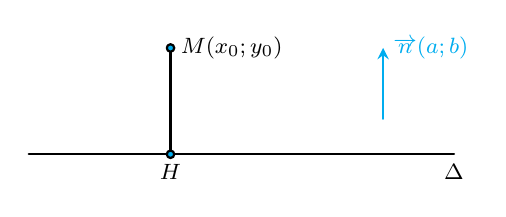
\begin{tikzpicture}[scale=.9, line join=round, line cap=round,font=\footnotesize,thick,>=stealth]
		\draw[-] (0,0)--(6,0) node [below]{$\Delta$};
		\draw (2,0) node [below]{$H$}--(2,1.5) node [right]{$M(x_0;y_0)$};
		\draw[fill=cyan] (2,0) circle(1.5pt) (2,1.5) circle(1.5pt);
		\draw[cyan,->] (5,0.5)--(5,1.5) node [right] {$\overrightarrow{n}(a;b)$};
	\end{tikzpicture}
}
\begin{vd}
	Tính khoảng cách từ điểm $M(2;4)$ đến đường thẳng $\Delta\colon 3x+4y-12=0$.
	\loigiai{
		Áp dụng công thức tính khoảng cách từ điểm $M$ đến đường thẳng $\Delta$, ta có
		$$
		\mathrm{d}(M,\Delta)=\dfrac{|3\cdot 2+4\cdot 4-12|}{\sqrt{3^2+4^2}}=\dfrac{10}{5}=2.
		$$
		Vậy khoảng cách từ điểm $M$ đến đường thẳng $\Delta$ là $2$.}
\end{vd}

\subsection{Các dạng toán thường gặp}
\begin{dang}{Vị trí tương đối của hai đường thẳng}
	\begin{center}
		Cho hai đường thẳng $\Delta_1\colon a_1x+b_1y+c_1=0$ và $ \Delta_2\colon a_2x+b_2y+c_2=0$.
	\end{center}
	\begin{itemize}
		\item $ \Delta_1$ cắt $ \Delta_2 \Leftrightarrow \dfrac{a_1}{a_2}\ne \dfrac{b_1}{b_2}$.
		\item $ \Delta_1\parallel \Delta_2 \Leftrightarrow \dfrac{a_1}{a_2}=\dfrac{b_1}{b_2}\ne \dfrac{c_1}{c_2}$.
		\item $ \Delta_1\equiv \Delta_2 \Leftrightarrow \dfrac{a_1}{a_2}=\dfrac{b_1}{b_2}=\dfrac{c_1}{c_2}$.
	\end{itemize}
	Chú ý rằng việc xét vị trí tương đối của hai đường thẳng cũng được xét qua số điểm chung của $\Delta$ và $\Delta'$. Việc xét vị trí tương đối và tính góc giữa hai đường thẳng cắt nhau cũng được thực hiện qua các vectơ chỉ phương của $\Delta$ và $\Delta'$.
\end{dang}
\begin{vd}%[0H3B1]
	Cho ba đường thẳng: $d_1: 2x+y-1=0$, $d_2: x+2y+1=0$, $d_3: mx-y-7=0$. Chứng minh rằng các đường thẳng $d_1, d_2$ cắt nhau và tìm giá trị của tham số $m$ để ba đường thẳng trên đồng quy.
	\loigiai{
		Ta có $\heva{&2x+y-1=0\\&x+2y+1=0}\Leftrightarrow \heva{&x=1\\&y=-1}$.\\
		Từ đó suy ra $d_1, d_2$ cắt nhau tại điểm $A(1;-1)$.\\
		Ba đường thẳng đã cho đồng quy khi và chỉ khi $d_3$ cũng đi qua điểm $A$, hay $A\in d_3$, suy ra
		$$m.1-(-1)-7=0 \Leftrightarrow m=6.$$
	}
\end{vd}

\begin{vd}%[0H3B1]
	Cho hai đường thẳng $\Delta: (m+3)x+3y-2m+3=0$ và $\Delta': 2x+2y+2-3m=0$. Tìm giá trị của tham số $m$ để\begin{enumerate}
		\item Đường thẳng $\Delta$ cắt đường thẳng $\Delta'$.
		\item 	Đường thẳng $\Delta$ song song với $\Delta'$.
	\end{enumerate}
	\loigiai{\begin{enumerate}
			\item
			$\Delta$ cắt $\Delta'$ khi và chỉ khi $\dfrac{m+3}{2}\neq \dfrac{3}{2}\Leftrightarrow m\neq 0$.\\
			\item	Theo câu a), để $\Delta$ song song với $\Delta'$ thì trước hết ta phải có $m=0$.\\
			Với $m=0$, khi đó dễ dàng nhận thấy $\Delta \equiv \Delta'$.\\
			Vậy không tồn tại $m$ để $\Delta \parallel \Delta'$.
		\end{enumerate}
		\emph{Chú ý}: Ta có thể làm theo cách sau: $\Delta$ song song với $\Delta'$ khi và chỉ khi $$\heva{\dfrac{m+3}{2}&=\dfrac{3}{2}\neq\dfrac{-2m+3}{2-3m}\\2-3m&\neq0}$$
		Hệ trên vô nghiệm, do đó không tồn tại $m$ để $\Delta \parallel \Delta'$.\\
	}
\end{vd}
\begin{vd}%[0H3B1]
	Cho ba đường thẳng: $d_1: 2x+y-1=0$, $d_2: x+2y+1=0$, $d_3: mx-y-7=0$. Chứng minh rằng các đường thẳng $d_1, d_2$ cắt nhau và tìm giá trị của tham số $m$ để ba đường thẳng trên đồng quy.
	\loigiai{
		Ta có $\heva{&2x+y-1=0\\&x+2y+1=0}\Leftrightarrow \heva{&x=1\\&y=-1}$.\\
		Từ đó suy ra $d_1, d_2$ cắt nhau tại điểm $A(1;-1)$.\\
		Ba đường thẳng đã cho đồng quy khi và chỉ khi $d_3$ cũng đi qua điểm $A$, hay $A\in d_3$, suy ra
		$$m.1-(-1)-7=0 \Leftrightarrow m=6.$$
	}
\end{vd}
\begin{vd}%[0H3K1]
	Cho các đường thẳng $\Delta: 2x+3y-5=0, \Delta': 3x-2y-1=0$ và điểm $M(2;3)$.\\
	a) Xét vị trí tương đối giữa các đường thẳng $\Delta$ và $\Delta'$.\\
	b) Biết $d$ là đường thẳng đi qua điểm $M$ và tạo với các đường thẳng $\Delta,\Delta'$ một tam giác cân. Tính góc giữa các đường thẳng $\Delta$ và $d$.
	\loigiai{
		a) Ta có $\vec{n}=(2,3)$ và $\vec{n'}=(3,-2)$ là các vectơ pháp tuyến của $\Delta$ và $\Delta'$.\\
		Ta thấy $\vec{n}$ và $\vec{n'}$ không cùng phương vì $\dfrac{2}{3}\neq \dfrac{3}{-2}$, từ đó suy ra $\Delta$ và $\Delta'$ là các đường thẳng cắt nhau.\\
		b) Ta có  $\vec{n}.\vec{n'}=2.3+3.(-2)=0$, do đó $\Delta$ và $\Delta'$ là các đường thẳng vuông góc với nhau.\\
		Gọi $A=\Delta\cap\Delta'$, $B=\Delta\cap d$, $C=d\cap\Delta'$. Khi đó tam giác $ABC$ là vuông tại $A$ do đó nếu tam giác $ABC$ cân thì $\widehat{B}=\widehat{C}=\dfrac{\pi}{4}$.\\
		Từ đó suy ra góc giữa các đường thẳng $\Delta$ và $d$ bằng $\dfrac{\pi}{4}$.
	}
\end{vd}

\begin{vd}
	Viết phương trình tổng quát của đường thẳng $\Delta$ qua  $A(1;2)$ và song song với đường thẳng $d\colon \heva{&x=-3+2t\\&y=-3t}(t\in\mathbb{R})$.
	%\dapso{$\Delta\colon 3x+2y-7=0$}
	\loigiai{
		Vì $\Delta \parallel d$ nên $\Delta$ nhận vectơ chỉ phương $\vec{u}=(2;-3)$ của $d$ làm vectơ chỉ phương. Do đó, $\Delta$ nhận $\vec{n}=(3;2)$ làm vectơ pháp tuyến.\\
		Vậy $\Delta$ có phương trình là $3(x-1)+2(y-2)=0$, hay $\Delta\colon 3x+2y-7=0$.
	}
\end{vd}
\begin{vd}
	Tìm $m$ sao cho hai đường thẳng $\Delta: x+5my-4=0$ và $\Delta': 2x+3y-2=0$ song song với nhau.
	\loigiai{
		$\Delta\parallel \Delta' \Leftrightarrow \dfrac{1}{2}=\dfrac{5m}{3}\ne\dfrac{-4}{-2}\Leftrightarrow m=\dfrac{3}{10}$.
	}
\end{vd}
\begin{vd}
	Trong mặt phẳng tọa độ $Oxy$, cho 3 đường thẳng $d_1$: $2x+y-4=0$, $d_2$: $5x-2y+3=0$, $d_3$: $mx+3y-2=0$.\begin{enumerate}
		\item Xét vị trí tương đối giữa $d_1$ và $d_2$.
		\item Tìm giá trị của tham số $m$ để 3 đường thẳng trên đồng quy.
	\end{enumerate}
	\loigiai{\begin{enumerate}
			\item Nhận thấy $\dfrac{2}{5}\neq \dfrac{1}{-2}$, từ đó suy ra các đường thẳng $d_1$, $d_2$ cắt nhau.
			\item Tọa độ giao điểm của hai đường thẳng $d_1$ và $d_2$ là nghiệm của hệ phương trình: $$\heva{2x+y-4&=0\\5x-2y+3&=0}\Leftrightarrow\heva{x&=\dfrac{5}{9}\\y&=\dfrac{26}{9}}.$$
			Vậy $d_1$ và $d_2$ cắt nhau tại điểm $M\left(\dfrac{5}{9};\dfrac{26}{9}\right)$.\\
			Vì $d_1$, $d_2$, $d_3$ đồng quy nên $M\in d_3$, ta có: $m.\dfrac{5}{9}+3.\dfrac{26}{9}-2=0$ $\Leftrightarrow$ $m=-12$
		\end{enumerate}
	}
\end{vd}



\begin{dang}{Bài toán liên quan đến góc giữa hai đường thẳng}
	\begin{itemize}
		\item Hai đường thẳng $a$ và $b$ cắt nhau tạo thành bốn góc. Số đo nhỏ nhất của các góc đó được gọi là số đo của góc giữa hai đường thẳng $a$ và $b$, hay đơn giản là góc giữa $a$ và $b$. Khi $a$ song song hoặc trùng với $b$, ta quy ước góc giữa chúng bằng $0^{\circ}$.
		\item Công thức xác định góc giữa hai đường thẳng:\\
		Góc xác định hai đường thẳng $ \Delta_1$ và $ \Delta_2$ có phương trình $ \Delta_1\colon a_1x+b_1y+c_1=0$ và $ \Delta_2\colon a_2x+b_2y+c_2=0$ được xác định bởi công thức $$\cos \left( \Delta_1; \Delta_2\right)=\dfrac{|a_1a_2+b_1b_2|}{\sqrt{a_1^2+b_1^2}\sqrt{a_2^2+b_2^2}}.$$
		\item Phương trình đường phân giác của góc tạo bởi hai đường thẳng $ \Delta_1\colon a_1x+b_1y+c_1=0$ và $ \Delta_2~\colon~ a_2x~+~b_2~y~+~c_2~=~0$ có phương trình
		$$\dfrac{a_1x+b_1y+c_1}{\sqrt{a_1^2+b_1^2}}=\pm \dfrac{a_2x+b_2y+c_2}{\sqrt{a_2^2+b_2^2}}.$$
	\end{itemize}
	
\end{dang}
\begin{vd}
	Trong mặt phẳng với hệ trục tọa độ $Oxy$ cho các đường thẳng $\Delta_1:x+2y-\sqrt{2}=0$ và $\Delta_2:x-y=0$. Tính côsin của góc giữa các đường thẳng $\Delta_1$ và $\Delta_2$.
	\loigiai{
		Ta có $\vec{n}=(1;2)$ và $\vec{n'}=(1;-1)$ là vectơ pháp tuyến của các đường thẳng $\Delta$ và $\Delta'$.\\
		Gọi $\varphi$ là góc giữa các đường thẳng $\Delta$ và $\Delta'$. Khi đó
		$$\cos\varphi = |\cos(\vec{n},\vec{n'})|=\dfrac{\sqrt{10}}{10}.$$
	}
\end{vd}
\begin{vd}
	Trong mặt phẳng với hệ trục tọa độ $Oxy$ cho các đường thẳng $\Delta\colon3x +5y + 15=0$ và $\Delta'\colon\heva{& x=10 - 3t\\& y=1 + 5t}$. Tính góc $\varphi$ giữa $\Delta_1$ và $\Delta_2$.
	\loigiai{
		Ta có $\vec{n}=(3;5)$ là một vectơ pháp tuyến của $\Delta$.\\
		$\vec{u'}=(-3;5)$ là một vectơ chỉ phương của $\Delta'$, suy ra $\Delta'$ có vectơ pháp tuyến $\vec{n'}=(5;3).$\\
		Do $\vec{n}\cdot\vec{n'}=0 \Rightarrow \Delta\bot \Delta'.$\\
		Vậy $\varphi=90^\circ$ 
	}
\end{vd}
\begin{vd}
	Trong mặt phẳng với hệ trục tọa độ $Oxy$ cho 2 đường thẳng $\Delta:x + 2y - 5=0$, $\Delta':3x + my - 1=0$. Tìm $m$ để góc giữa hai đường thẳng $\Delta$, $\Delta'$ bằng ${45}^{\circ}$.
	\loigiai{
		$\Delta: x + 2y - 5=0$ có vectơ pháp tuyến $\vec{n}=(1; 2)$,\\
		$\Delta': 3x + my - 1=0$ có vectơ pháp tuyến $\vec{n'}=(3; m)$.\\
		Theo bài ra ta có:
		$\cos45^{\circ}=\dfrac{\left|\vec{n}.\vec{n'}\right|}{\left|\vec{n}\right|. \left|\vec{n'}\right|}=\dfrac{\left|3 + 2m\right|}{\sqrt{5}\sqrt{3^2 + m^2}}.$\\
		Từ đó suy ra $\hoac{& m=1\\&m= - 9.}$\\
		Vậy với $\hoac{& m=1\\&m= - 9}$ thì góc giữa hai đường thẳng $\Delta$, $\Delta'$ bằng ${45}^{\circ}$.
	}
\end{vd}
\begin{dang}{Bài toán liên quan đến khoảng cách giữa hai đường thẳng}
	\begin{dl}[Công thức tính khoảng cách từ một điểm tới đường thẳng]
		Cho đường thẳng $ \Delta \colon ax+by+c=0$ và điểm $M(x_0;y_0)$. Khi đó khoảng cách từ $M$ đến $ \Delta $ được tính bởi công thức 
		\begin{equation*}
			\mathrm{d}\left(M, \Delta \right)=\dfrac{|ax_0+by_0+c|}{\sqrt{a^2+b^2}}.
		\end{equation*}
	\end{dl}
	\begin{hq}[Vị trí của hai điểm đối với đường thẳng]
		Cho đường thẳng và $M(x_M;y_M)\notin \Delta $, $N(x_N;y_N)\notin \Delta $. Khi đó
		\begin{itemize}
			\item $M, N$ cùng phía với $ \Delta $ khi và chỉ khi $(ax_M+by_M+c)(ax_N+by_N+c)>0$.
			\item $M, N$ khác phía với $ \Delta $ khi và chỉ khi $(ax_M+by_M+c)(ax_N+by_N+c)<0$.
		\end{itemize}
	\end{hq}
\end{dang}
\begin{vd}
	Tìm khoảng cách từ điểm $M(1;2)$ đến đường thẳng $(d)\colon 4x+3y-2=0$.
	\loigiai{
		Áp dụng công thức tính khoảng cách ta có\\
		$\mathrm{d}(M,D)=\dfrac{|4\cdot 1+3\cdot 2-2|}{\sqrt{4^2+3^2}}=\dfrac{8}{5}$.
	}
\end{vd}

\begin{vd}
	Tìm những điểm nằm trên đường thẳng $\Delta\colon 2x + y - 1 = 0$ và có khoảng cách đến $(d)\colon 4x + 3y - 10 = 0$ bằng $2$.
	\loigiai{
		Giả sử có điểm $M\in \Delta$, khi đó $M(m;1-2m)$.\\
		Theo đề $\mathrm{d}(M,\Delta)=2\Leftrightarrow \dfrac{|4m+3(1-2m)-10|}{\sqrt{4^2+3^2}}=2\Leftrightarrow |-2m-7|=10\\
		\Leftrightarrow \hoac{&2m+7=10\\&2m+7=-10}\Leftrightarrow\hoac{&m=\dfrac{3}{2}\\&m=-\dfrac{17}{2}.}$.\\
		Vậy có hai điểm thỏa mãn điều kiện là $M_1\left(\dfrac{3}{2};-2\right)$ và $M_2\left(-\dfrac{17}{2};18\right)$.
	}
\end{vd}

\begin{vd}
	Viết phương trình của đường thẳng đi qua điểm $A(1, -3)$ và có khoảng cách đến điểm $M_0(2, 4)$ bằng $1$.
	\loigiai{
		Giả sử đường thẳng $\Delta$ đi qua điểm $A(1;-3)$ có vectơ pháp tuyến là $\overrightarrow{n}=(a;b)$. Khi đó phương trình $\Delta$ có dạng
		$ax+by-a+3b=0$.\\
		Theo đề ta có\allowdisplaybreaks
		\begin{eqnarray*} &&\mathrm{d}(M_0,\Delta)=\dfrac{|2a+4b-a+3b|}{\sqrt{a^2+b^2}}=1\\
			&\Leftrightarrow& |a+7b|=\sqrt{a^2+b^2}\Leftrightarrow 
			48b^2+14ab=0\\
			&\Leftrightarrow& \hoac{&b=0\\&14a=-48b.}
		\end{eqnarray*}
		Với $b=0$ chọn $a=1$ ta có $\Delta\colon x-1=0$.\\
		Với $7a=-24b$ chọn $a=24\Rightarrow b=-7$ ta được $\Delta\colon 24x-7y-45=0$.
	}
\end{vd}

\begin{vd}
	Viết phương trình của đường thẳng $(d)$ song song với $(d’)\colon 3x + 4y - 1 = 0$ và cách $(d')$ một đoạn bằng $2$.
	\loigiai{
		Đường thẳng $(d)\parallel (d')$ nên phương trình đường thẳng $(d)\colon 3x+4y+c=0$.\\
		Lấy điểm $M(-1;1)\in (d')$, theo đề ta có:\\
		$\mathrm{d}(d,d')=\mathrm{d}(M,d)=2\Leftrightarrow \dfrac{|-3+4+c|}{5}=2\Leftrightarrow |c+1|=10\Leftrightarrow\hoac{&c=9\\&c=-11}$.\\
		Với $c=9$ ta có $d\colon 3x+4y+9=0$.\\
		Với $c=-11$ ta có $d\colon 3x+4y-11=0$.
	}
\end{vd}

\begin{vd}
	Cho điểm $A(-1,2)$ và hai đường $(\Delta)\colon x-y-1 = 0,(\Delta')\colon x+2y-5=0$. Tìm trên đường thẳng $(\Delta)$ một điểm $M$ sao cho khoảng cách từ $M$ đến $(\Delta')$ bằng $AM$.
	\loigiai{
		Ta có $M\in \Delta$, suy ra $M(m,m-1)$.\\
		$\vec{AM}=(m+1;m-3)\Rightarrow AM=\sqrt{(m+1)^2+(m-3)^2}=\sqrt{2m^2-4m+10}$.\\
		Theo đề\allowdisplaybreaks\begin{eqnarray*} &&\dfrac{|m+2(m-1)-5|}{\sqrt{5}}=\sqrt{2m^2-4m+10}\Leftrightarrow |3m-7|=\sqrt{5(2m^2-4m+10)}\\
			&\Leftrightarrow& (3m-7)^2=10m^2-20m+50\Leftrightarrow m^2+22m+1=0\\
			&\Leftrightarrow& m=-11\pm 2\sqrt{30}.
		\end{eqnarray*}
		Vậy có hai điểm thỏa mãn là $M_1(-11-2\sqrt{30};-12-2\sqrt{30})$ và $M_2(-11+2\sqrt{30};-12+2\sqrt{30})$.
	}
\end{vd}

\begin{vd}
	Cho tam giác $ABC$. Tính diện tích tam giác $ABC$, với  $A(-2; 14)$, $B(4; -2)$, $C(5; -4)$.
	\loigiai{
		Ta có $\vec{BC}=(1;-2)\Rightarrow BC=\sqrt{5}$. Phương trình đường thẳng $BC$ đi qua $B$ có dạng $2(x-4)+1(y+2)=0\Leftrightarrow 2x+y-6=0$.\\
		Đường cao $AH$ của tam giác $ABC$: $AH=\dfrac{|2(-2)+14-6|}{\sqrt{5}}=\dfrac{4\sqrt{5}}{5}$.\\
		Do đó $S_{ABC}=\dfrac{1}{2}\cdot AH\cdot BC=\dfrac{4\sqrt{5}\cdot \sqrt{5}}{10}=2$(đvdt).
	}
\end{vd}
\subsection{Bài tập tự luận}
%Bài 7.7
\begin{bt}%[0H3B1-3]
	Xét vị trí tương đối giữa các cặp đường thẳng sau:
	\begin{enumerate}
		\item $\Delta_{1}: 3 \sqrt{2} x+\sqrt{2} y-\sqrt{3}=0$ và $\Delta_{2}: 6 x+2 y-\sqrt{6}=0$.
		\item $d_{1}: x-\sqrt{3} y+2=0$ và $d_{2}: \sqrt{3} x-3 y+2=0$.
		\item $m_{1}: x-2 y+1=0$ và $m_{2}: 3 x+y-2=0$. 
	\end{enumerate}
	\loigiai{
		\begin{enumerate}
			\item Ta thấy $3 \sqrt{2} x+\sqrt{2} y-\sqrt{3}=0\Leftrightarrow 6 x+2 y-\sqrt{6}=0$ nên $\Delta_{1}\equiv \Delta_{2}$.
			\item Xét hệ phương trình $\heva{& x-\sqrt{3} y+2=0\\&\sqrt{3} x-3 y+2=0.}$\\
			Ta thấy hệ vô nghiệm nên $d_1$ và $d_2$ không có điểm chung, vậy chúng song song với nhau.
			\item Ta có $\heva{&x-2 y+1=0\\&3 x+y-2=0}\Leftrightarrow \heva{&x=\dfrac{3}{7}\\&y=\dfrac{5}{7}.}$\\
			Vậy hai đường thẳng $m_1$ và $m_2$ cắt nhau. 
		\end{enumerate}
	}
\end{bt}

\begin{bt}%[0H3B1-4]
	Tính góc giữa các cặp đường thẳng sau
	\begin{enumerate}
		\item $\Delta_{1}: \sqrt{3} x+y-4=0$ và $\Delta_{2}: x+\sqrt{3} y+3=0$;
		\item $d_{1}:\left\{\begin{array}{l}x=-1+2 t \\ y=3+4 t\end{array}\right.$ và $d_{2}:\left\{\begin{array}{l}x=3+s \\ y=1-3 s\end{array} \quad\right.$ (t, s là các tham số). 
	\end{enumerate}
	\loigiai{
		\begin{enumerate}
			\item Vectơ pháp tuyến của $\Delta_{1}$ là $\vec{n}_{1}=(\sqrt{3};1)$, của $\Delta_{2}$ là $\overrightarrow{n_{2}}=(1 ;\sqrt{3})$.
			Gọi $\varphi$ là góc giữa hai đường thẳng $\Delta_{1}$ và $\Delta_{2}$. Ta có
			$$
			\cos \varphi=\left|\cos \left(\overrightarrow{n_{1}}, \vec{n_{2}}\right)\right|=\dfrac{\left|\overrightarrow{n_{1}} \cdot \overrightarrow{n_{2}}\right|}{\left|\overrightarrow{n_{1}}\right| \cdot\left|\overrightarrow{n_{2}}\right|}=\dfrac{|\sqrt{3} \cdot 1+1 \cdot(\sqrt{3})|}{\sqrt{(\sqrt{3})^{2}+1^{2}} \cdot \sqrt{1^{2}+(\sqrt{3})^{2}}}=\dfrac{\sqrt{3}}{2} .
			$$
			Do đó, góc giữa $\Delta_{1}$ và $\Delta_{2}$ là $\varphi=30^{\circ}$.
			\item Vectơ chỉ phương của $d_{1}$ là $\vec{u}_{1}=(2;4)$, của $d_{2}$ là $\vec{u_{2}}=(1 ;-3)$.
			Gọi $\varphi$ là góc giữa hai đường thẳng $d_{1}$ và $d_{2}$. Ta có
			$$
			\cos \varphi=\left|\cos \left(\overrightarrow{u_{1}}, \overrightarrow{u_{2}}\right)\right|=\dfrac{\left|\overrightarrow{u_{1}} \cdot \overrightarrow{u_{2}}\right|}{\left|\overrightarrow{u_{1}}\right| \cdot\left|\overrightarrow{u_{2}}\right|}=\dfrac{|2 \cdot 1+4 \cdot(-3)|}{\sqrt{(2)^{2}+4^{2}} \cdot \sqrt{1^{2}+(-3)^{2}}}=\dfrac{\sqrt{2}}{2} .
			$$
			Do đó, góc giữa $d_{1}$ và $d_{2}$ là $\varphi=45^{\circ}$. 
		\end{enumerate}
		
	}
\end{bt}

\begin{bt}%[0H3B1-5]
	Trong mặt phẳng toạ độ $Oxy$, cho điểm $A(0;-2)$ và đường thẳng $\Delta\colon x+y-4=0$.
	\begin{enumerate}
		\item Tính khoảng cách từ điểm $A$ đến đường thẳng $\Delta$.
		\item Viết phương trình đường thẳng $a$ đi qua điểm $M(-1 ; 0)$ và song song với $\Delta$.
		\item Viết phương trình đường thẳng $b$ đi qua điểm $N(0 ; 3)$ và vuông góc với $\Delta$. 
	\end{enumerate}
	\loigiai{
		\begin{enumerate}
			\item Áp dụng công thức tính khoảng cách từ điểm $A$ đến đường thẳng $\Delta$, ta có
			$$
			\mathrm{d}(A, \Delta)=\dfrac{|0-2-4|}{\sqrt{1^{2}+1^{2}}}=3\sqrt{2}.
			$$
			Vậy khoảng cách từ điểm $A$ đến đường thẳng $\Delta$ là $3\sqrt{2}$.
			\item Đường thẳng $a$ đi qua điểm $M(-1; 0)$ và song song với $\Delta$ sẽ có vectơ pháp tuyến $\vec{n}=(1; 1)$ nên có phương trình $1(x+1)+1(y-0)=0\Leftrightarrow x+y=0$ (thỏa mãn).\\
			Vậy $a\colon x+y=0$.
			\item Viết phương trình đường thẳng $b$ đi qua điểm $N(0 ; 3)$ và vuông góc với $\Delta$ nên có vectơ pháp tuyến là $\vec{n}=(-1;1)$ nên có phương trình $$-1(x-0)+1(y-3)=0\Leftrightarrow -x+y-3=0$$.
			Vậy $b\colon -x+y-3=0$.
		\end{enumerate}
	}
\end{bt}

\begin{bt}%[0H3K1-5]
	Trong mặt phẳng toạ độ, cho tam giác $ABC$ có $A(1; 0), B(3 ; 2)$ và $C(-2 ;-1)$.
	\begin{enumerate}
		\item Tính độ dài đường cao kẻ từ đỉnh $A$ của tam giác $ABC$.
		\item Tính diện tích tam giác $ABC$. 
	\end{enumerate}
	\loigiai{
		\begin{enumerate}
			\item Đường thẳng $BC$ qua $B(3; 2)$ và nhận $\vec{BC}=(-5; -3)$ làm vectơ chỉ phương nên có vectơ pháp tuyến là $\vec{n}=(3; -5)$. Suy ra đường thẳng $BC$ có phương trình $3(x-3)-5(y-2)=0\Leftrightarrow 3x-5y-1=0$.\\
			Độ dài đường cao kẻ từ đỉnh $A$ của $\triangle ABC$ chính bằng $\mathrm{d}(A,BC)=\dfrac{2}{\sqrt{34}}$.
			\item Ta có $BC=\sqrt{34}$, suy ra diện tích tam giác $ABC$ là $$S_{\triangle ABC}=\dfrac{1}{2}BC\cdot \mathrm{d}(A,BC)=\dfrac{1}{2}\cdot \sqrt{34}\cdot\dfrac{2}{\sqrt{34}}=1.$$ 
		\end{enumerate}
		
	}
\end{bt}

\begin{bt}%[0H3K1-3]
	Chứng minh rằng hai đường thẳng $d: y=ax+b$ $(a \neq 0)$ và $d': y=a' x+b'\left(a' \neq 0\right)$ vuông góc với nhau khi và chỉ khi $a a'=-1$.
	\loigiai{Ta có $d\colon y=ax+b\Leftrightarrow ax-y+b=0$ nên $d$ có vectơ pháp tuyến $\vec{n}=(a;-1)$.\\
		Tương tự $d'$ có vectơ pháp tuyến $\vec{n'}=(a'; -1)$.\\
		Vậy $d\perp d'\Leftrightarrow \vec{n}\cdot \vec{n'}=0\Leftrightarrow aa'+1=0\Leftrightarrow aa'=-1$.\\
		Suy ra điều phải chứng minh.
	}
\end{bt}

\begin{bt}%[0H3K1-5]
	Trong mặt phẳng toạ độ, một tín hiệu âm thanh phát đi từ một vị trí và được ba thiết bị ghi tín hiệu đặt tại ba vị trị $O(0 ; 0), A(1 ; 0), B(1 ; 3)$ nhận được cùng một thời điểm. Hãy xác định vị trí phát tín hiệu âm thanh.
	\loigiai{
		Gọi $I$ là vị trí phát tín hiệu âm thanh đó, từ giả thiết suy ra $IA=IB=IO$ nên $I$ chính là tâm đường tròn ngoại tiếp của tam giác $OAB$.\\
		Đặt $I(a; b)$ ta có 
		\begin{eqnarray*}
			IA=IB=IO&\Leftrightarrow& \heva{&IA=IO\\&IB=IO}\Leftrightarrow \heva{&(a-1)^2+b^2=a^2+b^2\\&(a-1)^2+(b-3)^2=a^2+b^2}\\
			&\Leftrightarrow& \heva{&-2a+1=0\\&-2a-6b+10=0}\Leftrightarrow \heva{&a=\dfrac{1}{2}\\&b=\dfrac{3}{2}.}	
		\end{eqnarray*}
		Vậy vị trí phát tín hiệu âm thanh là $I\left(\dfrac{1}{2};\dfrac{3}{2}\right)$.}
\end{bt}

\begin{bt}%[Dự án BG-5]%[Quảng Đại Mưa]%[0H3Y1-2]
	Lập phương trình tham số, phương trình chính tắc (nếu có) và phương trình tổng quát của
	đường thẳng đi qua điểm $A$ và có vectơ pháp tuyến $\overrightarrow{n}$. 
	\begin{listEX}[1]
		\item $A(0;1)$, $\overrightarrow{n} = (1;3)$.   
		%\dapso{$\heva{&x=3 t\\&y=1-t}$; $\dfrac{x}{3} =\dfrac{y-1}{-1}$; $x+3y-3=0$}
		\loigiai{
			Đường thẳng đi qua $A(0;1)$ và có vectơ pháp tuyến $\overrightarrow{n} = (1;3)$ nên có phương trình tổng quát là
			\[1(x-0)+3(y-1) =0 \Leftrightarrow x+3y -3=0.\] 
			Đường thẳng có vectơ chỉ phương là $\overrightarrow{u} = (3;-1)$ và đi qua $A(0;1)$ nên có phương trình tham số và chính tắc là 
			\[
			\heva{&x=3 t\\&y=1-t} ; \quad \dfrac{x}{3} =\dfrac{y-1}{-1}. 
			\]
		}
		\item $A(-2;3)$, $\overrightarrow{n} = (5;-1)$.   
		%\dapso{$\heva{&x=-2+ t\\&y=3+5t}$; $\dfrac{x+2}{1} =\dfrac{y-3}{5}$; $5x-y+13=0$}
		\loigiai{
			Đường thẳng đi qua $A(-2;3)$ và có vectơ pháp tuyến $\overrightarrow{n} = (5;-1)$ nên có phương trình tổng quát là
			\[5(x+2)-(y-3) =0 \Leftrightarrow 5x-y +13=0.\] 
			Đường thẳng có vectơ chỉ phương là $\overrightarrow{u} = (1;5)$ và đi qua $A(-2;3)$ nên có phương trình tham số và chính tắc là 
			\[
			\heva{&x=-2+ t\\&y=3+5t} ; \quad \dfrac{x+2}{1} =\dfrac{y-3}{5}. 
			\]
		}
		
	\end{listEX}
\end{bt}


\begin{bt}%[Dự án BG-5]%[Quảng Đại Mưa]%[0H3Y1-2]
	Lập phương trình tham số, phương trình chính tắc (nếu có) và phương trình tổng quát của
	đường thẳng đi qua điểm $A$ và có hệ số góc $k$. 
	\begin{listEX}[1]
		\item  $A(2;4)$, $k=2$.  
		%\dapso{$\heva{&x= 2+t\\&y=4+2t}$; $\dfrac{x-2}{1} =\dfrac{y-4}{2}$; $2x-y =0$}
		\loigiai{
			Đường thẳng đi qua $A(2;4)$ và có hệ số góc $k=2$ nên có phương trình  $y= 2(x-2)+4$, do đó có phương  trình tổng quát là $2x-y=0$. Khi đó, đường thẳng có vectơ chỉ phương $\overrightarrow{u} = (1;2)$. Đường thẳng có phương trình tham số và chính tắc là
			\[
			\heva{&x= 2+t\\&y=4+2t} ; \quad \dfrac{x-2}{1} =\dfrac{y-4}{2}. 
			\]
		}
		\item  $A(-3;1)$, $k=-2$.  
		%\dapso{$\heva{&x= -3+t\\&y=1-2t}$; $\dfrac{x+3}{1} =\dfrac{y-1}{-2}$; $2x+y+5=0$}
		\loigiai{
			Đường thẳng đi qua $A(-3;1)$ và có hệ số góc $k=-2$ nên có phương trình  $y= -2(x+3)+1$. \\ 
			Do đó có phương  trình tổng quát là $2x+y+5=0$. \\
			Khi đó, đường thẳng có vectơ chỉ phương $\overrightarrow{u} = (1;-2)$. \\
			Đường thẳng có phương trình tham số  là $\heva{&x= -3+t\\&y=1-2t.}$  \\
			Đường thẳng có phương trình chính tắc là $\dfrac{x+3}{1} =\dfrac{y-1}{-2}$. 
			
		}
		
	\end{listEX}
\end{bt}

\begin{bt}%[Dự án BG-5]%[Quảng Đại Mưa]%[0H3B1-2]
	Lập phương trình tham số, phương trình chính tắc (nếu có) và phương trình tổng quát của đường thẳng đi qua hai điểm $A$ và $B$.
	\begin{listEX}[1]
		\item  $A(2;1)$, $B(-4;5)$. 
		%\dapso{$\heva{&x= 2 -3t\\&y=1+2t}$; $\dfrac{x-2}{-3} =\dfrac{y-1}{2}$; $2x+3y-7=0$}
		\loigiai{
			Ta có $\overrightarrow{AB} = (-6;4)$. \\
			Đường thẳng có vectơ pháp tuyến $\overrightarrow{n}= (2;3)$, vectơ chỉ phương $\overrightarrow{u}= (-3;2)$ và đi qua $A$ suy ra \\
			Phương trình tham số $\heva{&x= 2 -3t\\&y=1+2t.}$ \\
			Phương trình chính tắc  $\dfrac{x-2}{-3} =\dfrac{y-1}{2}.$ \\
			Phương trình tổng quát $2x+3y-7=0$.
		}
		\item  $A(5;3)$, $B(-2;-7)$. 
		%\dapso{$\heva{&x= 5 +7t\\&y=3+10t}$; $\dfrac{x-5}{7} =\dfrac{y-3}{10}$; $10x-7y-29=0$}
		\loigiai{
			Ta có $\overrightarrow{AB} = (-7;-10)$. \\
			Đường thẳng có vectơ pháp tuyến $\overrightarrow{n}= (10;-7)$, vectơ chỉ phương $\overrightarrow{u}= (7;10)$ và đi qua $A$ suy ra \\
			Phương trình tham số $\heva{&x= 5 +7t\\&y=3+10t.}$ \\
			Phương trình chính tắc   $\dfrac{x-5}{7} =\dfrac{y-3}{10}$.\\
			Phương trình tổng quát $10x-7y-29=0$.
		}
		
	\end{listEX}
\end{bt}
\begin{bt}%[Dự án BG-5]%[Quảng Đại Mưa]%[0H3B1-3]
	Xét vị trí tương đối của cặp đường thẳng $d_1\colon 2x+3y+1=0$ và $d_2\colon 4x+5y-6=0$. Tìm tọa độ giao điểm nếu chúng cắt nhau.
	%\dapso{Hai đường thẳng cắt nhau tại điểm $M\left(\dfrac{23}{2};-8\right)$}
	\loigiai
	{Xét hệ phương trình $\heva{&2x+3y=-1\\&4x+5y=6} \Leftrightarrow \heva{&x=\dfrac{23}{2}\\&y=-8.}$\\
		Hệ phương trình có nghiệm duy nhất nên hai đường thẳng cắt nhau, tọa độ giao điểm là $M\left(\dfrac{23}{2};-8\right)$.}
\end{bt}

\begin{bt}%[Dự án BG-5]%[Quảng Đại Mưa]%[0H3B1-3]
	Xét vị trí tương đối của cặp đường thẳng $d_1\colon \heva{&x=5+t\\&y=-1}$ và $d_2\colon x+y-5=0$. Tìm tọa độ giao điểm nếu chúng cắt nhau.
	%\dapso{Hai đường thẳng $d_1$ và $d_2$ cắt nhau tại điểm $M(6;-1)$}
	\loigiai
	{Xét hệ phương trình $\heva{&x=5+t\\&y=-1\\&x+y-5=0} \Leftrightarrow \heva{&x=6\\&y=-1\\&t=1}$.\\
		Hệ phương trình có nghiệm duy nhất $(x;y;t)$ là $(6;-1;1)$, do đó hai đường thẳng $d_1$ và $d_2$ cắt nhau tại điểm $M(6;-1)$.}
\end{bt}






\begin{bt}%[Dự án BG-5]%[Quảng Đại Mưa]%[0H3B1-4]
	Tính góc giữa hai đường thẳng $d_1\colon x-2y-1=0$ và $d_2\colon x+3y-11=0$.
	%\dapso{$(d_1,d_2)=45^\circ$}
	\loigiai
	{Đường thẳng $d_1$ có vectơ pháp tuyến $\vec{n}_1=(1;-2)$, đường thẳng $d_2$ có vectơ pháp tuyến $\vec{n}_2=(1;3)$, do đó
		$$\cos(d_1,d_2)=\left|\cos\left(\vec{n}_1,\vec{n}_2\right)\right|=\dfrac{\left|\vec{n}_1\cdot \vec{n}_2\right|}{\left|\vec{n}_1\right|\cdot\left|\vec{n}_2\right|} = \dfrac{|1-6|}{\sqrt{5}\cdot\sqrt{10}}=\dfrac{1}{\sqrt{2}} \Rightarrow (d_1,d_2)=45^\circ.$$}
\end{bt}

\begin{bt}%[Dự án BG-5]%[Quảng Đại Mưa]%[0H3B1-5]
	Tính khoảng cách từ điểm $M(4;-5)$ đến đường thẳng $d\colon \heva{&x=2t\\&y=2+3t}$.
	%\dapso{$\mathrm{d}(M,d)=2\sqrt{13}$}
	\loigiai{Đường thẳng $d\colon \heva{&x=2t\\&y=2+3t}$ qua điểm $A(0;2)$, có vectơ chỉ phương $\vec{u}=(2;3)$ nên phương trình tổng quát của $d$ là
		$$3x-2(y-2)=0 \Leftrightarrow 3x-2y+4=0.$$
		Khoảng cách từ điểm $M(4;-5)$ đến đường thẳng $d$ bằng
		$$\mathrm{d}(M,d)=\dfrac{\left|3\cdot 4-2\cdot(-5)+4\right|}{\sqrt{9+4}}=\dfrac{26}{\sqrt{13}}=2\sqrt{13}.$$}
\end{bt}
\begin{bt}%[Dự án BG-5]%[Quảng Đại Mưa]%[0H3B1-2]
	Viết phương trình các đường phân giác của các góc tạo bởi hai đường thẳng $d_1\colon 3x-4y+12=0$ và $d_2\colon 12x+5y-20=0$.
	%\dapso{$21x+77y-256=0$, $99x-27y+56=0$}
	\loigiai
	{Điểm $M(x;y)$ nằm trên đường phân giác của góc tạo bởi hai đường thẳng $d_1$, $d_2$ khi và chỉ khi
		\begin{align*}
			\mathrm{d}(M,d_1)&=\mathrm{d}(M,d_2)\\
			&\Leftrightarrow \dfrac{|3x-4y+12|}{\sqrt{9+16}}=\dfrac{|12x+5y-20|}{\sqrt{144+25}}\\
			&\Leftrightarrow 13|3x-4y+12|=5|12x+5y-20|\\
			&\Leftrightarrow \hoac{&21x+77y-256=0 \\&99x-27y+56=0.}
		\end{align*}
		Vậy phương trình các đường phân giác của góc giữa hai đường thẳng $d_1$ và $d_2$ là $21x+77y-256=0$ và $99x-27y+56=0$.}
\end{bt}
\begin{bt}%[Tex hoa sach Toan 10]%[Đỗ Đường Hiếu]%[0H3B1-3]
	Xét vị trí tương đối của mỗi cặp đường thẳng sau
	\begin{enumerate}
		\item $d_1\colon 3x+2y-5=0$ và $d_2\colon x-4y+1=0$;
		\item $d_3\colon x-2y+3=0$ và $d_4\colon -2x+4y+10=0$;
		\item $d_5\colon 4x+2y-3=0$ và $d_6\colon\heva{&x=-\dfrac{1}{2}+t\\&y=\dfrac{5}{2}-2t.}$
	\end{enumerate}
	\loigiai{
		\begin{enumerate}
			\item Đường thẳng $d_1$ có vectơ chỉ phương $\overrightarrow{u}_1=(2;-3)$, đường thẳng $d_2$ có vectơ chỉ phương $\overrightarrow{u}_2=(4;1)$.\\
			Do $\dfrac{2}{4}\ne \dfrac{-3}{1}$ nên $\overrightarrow{u}_1$, $\overrightarrow{u}_2$ không cùng phương, suy ra $d_1$ cắt $d_2$.
			\item Đường thẳng $d_3$ có vectơ chỉ phương $\overrightarrow{u}_3=(2;1)$, đường thẳng $d_4$ có vectơ chỉ phương $\overrightarrow{u}_4=(4;2)$. Suy ra $\overrightarrow{u}_4=2\overrightarrow{u}_3$.\\
			Ta có điểm $M(-1;1)\in d_3$. Do $-2\cdot (-1)+4\cdot 1+10\ne 0$ nên $M(-1;1)\notin d_4$.\\
			Vậy $d_3$ song song với $d_4$.
			\item Đường thẳng $d_5$ có vectơ chỉ phương $\overrightarrow{u}_5=(2;-4)$, đường thẳng $d_6$ có vectơ chỉ phương $\overrightarrow{u}_2=(1;-2)$. Suy ra $\overrightarrow{u}_5=2\overrightarrow{u}_6$.\\
			Ta có điểm $N\left(-\dfrac{1}{2};\dfrac{5}{2}\right) \in d_6$. Do $4\cdot \left(-\dfrac{1}{2}\right) +2\cdot\left(\dfrac{5}{2}\right)-3= 0$ nên $N\left(-\dfrac{1}{2};\dfrac{5}{2}\right) \in d_5$.\\
			Vậy $d_5$ và $d_6$ trùng nhau.
		\end{enumerate}
	}
\end{bt}

\begin{bt}%[Tex hoa sach Toan 10]%[Đỗ Đường Hiếu]%[0H3B1-4]
	Tính số đo góc giữa hai đường thẳng $d_1\colon 2x-y+5=0$ và $d_2\colon x-3y+3=0$.
	\loigiai{
		$d_1$ có vectơ pháp tuyến $\overrightarrow{n}_1=(2;-1)$, $d_2$ có vectơ pháp tuyến $\overrightarrow{n}_2=(1;-3)$. Do đó, ta có
		\[\cos \left(d_1,d_2\right)=\left|\cos \left(\overrightarrow{n}_1,\overrightarrow{n}_2\right)\right|=\dfrac{\left|\overrightarrow{n}_1\cdot \overrightarrow{n}_2\right|}{\left|\overrightarrow{n}_1\right|\cdot \left|\overrightarrow{n}_2\right|}=\dfrac{\left|2\cdot 1+(-1)\cdot (-3)\right|}{\sqrt{2^2+(-1)^2}\cdot \sqrt{1^2+(-3)^2}}=\dfrac{1}{\sqrt{2}}.\]
		Vậy $\left(d_1,d_2\right)=45^\circ$.
	}	
\end{bt}

\begin{bt}%[0H3B1-5]
	Tính khoảng cách từ một điểm đến một đường thẳng trong mỗi trường hợp sau
	\begin{enumerate}
		\item $A(1;-2)$ và $\Delta_1\colon 3x-y+4=0$;
		\item $B(-3;2)$ và $\Delta_2\colon \heva{&x=-2+t\\&y=1-2t.}$
	\end{enumerate}
	\loigiai{
		\begin{enumerate}
			\item Ta có
			\[\mathrm{d}\left(A,\Delta_1\right)=\dfrac{\left|3\cdot 1-(-2)+4\right|}{\sqrt{3^2+(-1)^2}}=\dfrac{9\sqrt{10}}{10}.\]
			\item Đường thẳng $\Delta_2$ đi qua điểm $M(-2;1)$ và có vectơ pháp tuyến $\overrightarrow{n}=(2;1)$.\\
			Phương trình tổng quát của đường thẳng $\Delta_2$ là
			\[2\cdot (x+2)+1\cdot (y-1)=0\Leftrightarrow 2x+y+2=0.\]
			Vậy $\mathrm{d}\left(B,\Delta_2\right)=\dfrac{\left|2\cdot (-3)+2+2\right|}{\sqrt{2^2+1^2}}=\dfrac{2\sqrt{5}}{5}$.
		\end{enumerate}
	}	
\end{bt}

\begin{bt}%[Tex hoa sach Toan 10]%[Đỗ Đường Hiếu]%[0H3B1-4]
	Với giá trị nào của tham số $m$ thì hai đường thẳng sau đây vuông góc?\\
	\centerline{$\Delta_1\colon mx-y+1=0$ và $\Delta_2\colon 2x-y+3=0$.}
	\loigiai{
		Hai đường thẳng $\Delta_1$ và $\Delta_2$ vuông góc với nhau khi và chỉ khi
		\[m\cdot 2+(-1)\cdot (-1)=0\Leftrightarrow m=-\dfrac{1}{2}.\]
	}	
\end{bt}

\begin{bt}%[Tex hoa sach Toan 10]%[Đỗ Đường Hiếu]%[0H3B1-4]
	Cho ba điểm $A(2;-1)$, $B(1;2)$ và $C(4;-2)$. Tính số đo góc $BAC$ và góc giữa hai đường thẳng $AB$, $AC$.
	\loigiai{
		Ta có $\overrightarrow{AB}=(-1;3)$, $\overrightarrow{AC}=(2;-1)$. Khi đó
		\[\cos \widehat{BAC}=\cos \left(\overrightarrow{AB},\overrightarrow{AC}\right)=\dfrac{(-1)\cdot 2+3\cdot (-1)}{\sqrt{(-1)^2+3^2}\cdot \sqrt{2^2+(-1)^2}}=-\dfrac{1}{\sqrt{2}}.\]
		Suy ra $\widehat{BAC}=135^\circ$. Từ đó ta có góc giữa hai đường thẳng $AB$, $AC$ bằng $45^\circ$.
	}	
\end{bt}

\begin{bt}%[Tex hoa sach Toan 10]%[Đỗ Đường Hiếu]%[0H3K1-5]
	Cho ba điểm $A(2;4)$, $B(-1;2)$ và $C(3;-1)$. Viết phương trình đường thẳng đi qua $B$ đồng thời cách đều $A$ và $C$.
	\loigiai{
		Phương trình đường thẳng đi qua điểm $B(-1;2)$ có dạng 
		\[\Delta\colon a\cdot(x+1)+b\cdot (y-2)=0\]
		với $a^2+b^2\ne 0$.\\
		$\Delta$ cách đều $A$ và $C$ khi và chỉ khi
		\allowdisplaybreaks
		\begin{eqnarray*}
			\mathrm{d}(A,\Delta)=\mathrm{d}(C,\Delta)
			&\Leftrightarrow& \dfrac{\left|a\cdot (2+1)+b\cdot (4-2)\right|}{\sqrt{a^2+b^2}}=\dfrac{\left|a\cdot (3+1)+b\cdot (-1-2)\right|}{\sqrt{a^2+b^2}}\\
			&\Leftrightarrow& \left|3a+2b\right|=\left|4a-3b\right|\\
			&\Leftrightarrow& \hoac{&3a+2b=4a-3b\\&3a+2b=-(4a-3b)}\\
			&\Leftrightarrow& \hoac{&a=5b\\&7a=b.}
		\end{eqnarray*}
		\begin{itemize}
			\item Với $a=5b$, chọn $a=5$ và $b=1$ ta có phương trình đường thẳng cần lập là
			\[5\cdot(x+1)+1\cdot (y-2)=0\Leftrightarrow 5x+y+3=0.\]
			\item Với $7a=b$, chọn $a=1$ và $b=7$ ta có phương trình đường thẳng cần lập là
			\[1\cdot(x+1)+7\cdot (y-2)=0\Leftrightarrow x+7y-13=0.\]
		\end{itemize}
		Vậy, có hai đường thẳng thỏa mãn đề bài là $5x+y+3=0$ và $x+7y-13=0$.
	}	
\end{bt}

\begin{bt}%[Tex hoa sach Toan 10]%[Đỗ Đường Hiếu]%[0H3T1-7]
	Có hai con tàu $A$ và $B$ cùng xuất phát từ hai bến, chuyển động đều theo đường thẳng ngoài biển. Trên màn hình ra-đa của trạm điều khiển (được coi như mặt phẳng tọa độ $Oxy$ với đơn vị trên các trục tính theo ki-lô-mét), tại thời điểm $t$ (giờ), vị trí của tàu $A$ có tọa độ được xác định bởi công thức $\heva{&x=3-33t\\&y=-4+25t}$, vị trí của tàu $B$ có tọa độ là $(4-30t;3-40t)$.
	\begin{enumerate}
		\item Tính cô-sin góc giữa hai đường đi của hai tàu $A$ và $B$.
		\item Sau bao lâu kể từ thời điểm xuất phát hai tàu gần nhau nhất?
		\item Nếu tàu $A$ đứng yên ở vị trí ban đầu, tàu $B$ chạy thì khoảng cách ngắn nhất giữa hai tàu bằng bao nhiêu?
	\end{enumerate}
	\loigiai{
		\begin{enumerate}
			\item Đường thẳng mà tàu $A$ đi có phương trình $d_1\colon \heva{&x=3-33t_1\\&y=-4+25t_1.}$\\
			Đường thẳng mà tàu $B$ đi có phương trình $d_2\colon \heva{&x=4-30t_2\\&y=3-40t_2.}$\\
			Đường thẳng $d_1$ có vectơ chỉ phương $\overrightarrow{u}_1=(-33;25)$, đường thẳng $d_2$ có vectơ chỉ phương $\overrightarrow{u}_2=(-30;-40)$. Do đó
			\[\cos \left(d_1,d_2\right)=\dfrac{\left|(-33)\cdot (-30)+25\cdot (-40) \right|}{\sqrt{(-33)^2+25^2}\cdot \sqrt{(-30)^2+(-40)^2}}=\dfrac{1}{5\sqrt{1714}}.\]
			\item Tại thời điểm $t$ (giờ), vị trí của tàu $A$ và tàu $B$ lần lượt là $M(3-33t;-4+25t)$ và $N(4-30t;3-40t)$.\\
			Do đó $MN=\sqrt{(3t+1)^2+(7-65t)^2}=\sqrt{4234t^2-904t+50}$.\\
			$MN$ ngắn nhất khi và chỉ khi hàm số $f(t)=4234t^2-904t+50$ đạt giá trị nhỏ nhất. Vì $f(t)$ là hàm số bậc hai nên $f(t)$ đạt giá trị nhỏ nhất tại $t=\dfrac{904}{2\cdot 4234}=\dfrac{226}{2117}$.\\
			Vậy, sau $\dfrac{226}{2117}$ giờ sau khi xuất phát, hai tàu $A$, $B$ ở gần nhau nhất.
			\item Vị trí ban đầu của tàu $A$ ứng với $t=0$ là điểm có tọa độ $H(3;-4)$.\\
			Đường thẳng $d_2$ có phương trình tổng quát là
			\[40\cdot (x-4)-30\cdot (y-3)=0\Leftrightarrow 4x-3y+7=0.\]
			Khi tàu $A$ đứng yên ở vị trí ban đầu, tàu $B$ chạy thì khoảng cách ngắn nhất giữa hai tàu bằng khoảng cách từ điểm $H$ đến đường thẳng $d_2$. Khoảng cách đó bằng
			\[\mathrm{d}(H,d_2)=\dfrac{\left|4\cdot 2-3\cdot (-4)+7\right|}{\sqrt{4^2+(-3)^2}}=5{,}4 \,(\text{km}).\]
		\end{enumerate}	
	}	
\end{bt}
\Closesolutionfile{ans}
\Closesolutionfile{ansbook}
\subsection{Bài tập trắc nghiệm}
\Opensolutionfile{ans}
\setcounter{ex}{0}
\begin{ex}%[BG5- Đình Nguyên]%[0H3Y1-1]
	Cho đường thẳng $d\colon 3x-2y+1=0$. Vectơ nào sau đây là một vectơ pháp tuyến $d$?
	\choice
	{$\overrightarrow{n}=(3;2)$}
	{$\overrightarrow{n}=(2;3)$}
	{\True $\overrightarrow{n}=(-3;2)$}
	{$\overrightarrow{n}=(-2;3)$}
	\loigiai{
		Ta có $\overrightarrow{n}=(-3;2)$ là một vectơ pháp tuyến của $d$.
	}
\end{ex}
\begin{ex}%[BG5- Đình Nguyên]%[0H3Y1-1]
	Nếu $d$ là đường thẳng vuông góc với $\Delta\colon 3x-2y+1=0$ thì $d$ có một	vec-tơ chỉ phương là
	\choice
	{$(2;3)$}
	{$(3;2)$}
	{$(-2;3)$}
	{\True $(6;-4)$}
	\loigiai{
		Ta có $\overrightarrow{n}=(3;-2)$ là một vectơ pháp tuyến của $\Delta$. Vì $\Delta\perp d$ nên mọi vectơ pháp tuyến của $\Delta$ đều là vectơ chỉ phương của $d$. Do đó $2\overrightarrow{n}=(6;-4)$ là một vectơ chỉ phương của $d$.
	}	
\end{ex}
\begin{ex}%[BG5- Đình Nguyên]%[0H3Y1-2]
	Viết phương trình đường thẳng $\Delta$ đi qua điểm $M(5;0)$ và có véc
	tơ pháp tuyến $\overrightarrow{n}=(1;-3)$.
	\choice
	{$x-3y+5=0$}
	{\True $x-3y-5=0$}
	{$3x-y-15=0$}
	{$3x+y-15=0$}
	\loigiai{
		Đường thẳng qua $M(5;0)$ và có vectơ pháp tuyến $\overrightarrow{n}=(1;-3)$ có phương trình là
		$$ 1x-3y-(1\cdot 5-3\cdot 0)=0\Leftrightarrow x-3y-5=0. $$	
	}	
\end{ex}
\begin{ex}%[BG5- Đình Nguyên]%[0H3Y1-2]
	Phương trình tổng quát của đường thẳng đi qua hai điểm $A(-2;4),B(1;0)$ là
	\choice
	{$4x+3y+4=0$}
	{$4x-3y+4=0$}
	{$4x-3y-4=0$}
	{\True $4x+3y-4=0$}
	\loigiai{
		Ta có $\overrightarrow{AB}=(3;-4)$ là một vectơ chỉ phương của đường thẳng $AB$. Suy ra $\overrightarrow{n}=(4;3)$ là một vectơ pháp tuyến của $AB$. Đường thẳng $AB$ có vectơ pháp tuyến $\overrightarrow{n}$ và đi qua $B$, suy ra phương trình đường thẳng $AB$ là
		$$ 4x+3y-(4\cdot1+3\cdot0)=0\Leftrightarrow 4x+3y-4=0. $$ 	
	}	
\end{ex}
\begin{ex}%[BG5- Đình Nguyên]%[0H3B1-2]
	Phương trình đường trung trực của đoạn AB với $A(1;5),B(-3;2)$ là
	\choice
	{$6x+8y+13=0$}
	{$-8x+6y-13=0$}
	{$8x+6y+13=0$}
	{\True $8x+6y-13=0$}
	\loigiai{
		Gọi $\Delta$ là đường trung trực của $AB$. Khi đó $\Delta$ nhận vectơ $\overrightarrow{BA}=(4;3)$ là vectơ pháp tuyến. Hơn nữa, trung điểm $M$ của đoạn $AB$ thuộc $\Delta$. Điểm $M$ có tọa độ là $\left(\dfrac{1+(-3)}{2};\dfrac{5+2}{2} \right) \Rightarrow M\left( -1;\dfrac72 \right)$. Suy ra phương trình đường thẳng $\Delta$ là
		$$ 4x+3y-\left( 4\cdot (-1)+3\cdot \dfrac72 \right)=0\Leftrightarrow 8x+6y-13=0. $$
	}
\end{ex}
\begin{ex}%[BG5- Đình Nguyên]%[0H3B1-2]
	Đường thẳng $d\colon \heva{&x=3-5t\\&y=1+4t}$ có phương trình tổng quát là
	\choice
	{\True $4x+5y-17=0$}
	{$4x+5y+17=0$}
	{$4x-5y+17=0$}
	{$4x-5y-17=0$}
	\loigiai{
		Ta có $\overrightarrow{u}=(-5;4)$ là một vectơ chỉ phương của $d$. Suy ra $\overrightarrow{n}=(4;5)$ là một vectơ pháp tuyến của $d$. Từ phương trình tham số của $d$ ta suy ra $$ 4x+5y=4(3-5t)+5(1+4t)=12-20t+5+20t=17. $$
		Suy ra $4x+5y=17\Leftrightarrow 4x+5y-17=0$.
	}	
\end{ex}
\begin{ex}%[BG5- Đình Nguyên]%[0H3Y1-4]
	Tính góc giữa hai đường thẳng $d_1 \colon 4x-2y+5=0$ và $d_2 \colon x-3y+1=0$.
	\choice
	{$60^\circ$}
	{$135^\circ$}
	{$30^\circ$}
	{\True $45^\circ$}
	\loigiai{
		Ta có $$\cos (d_1,d_2)=\dfrac{|4\cdot 1+(-2)\cdot(-3)|}{\sqrt{4^2+(-2^2)}\cdot\sqrt{1^2+(-3)^2}}=\dfrac{10}{10\sqrt{2}}=\dfrac{1}{\sqrt{2}}.$$	Suy ra $(d_1,d_2)=45^\circ$.
	}	
\end{ex}
\begin{ex}%[BG5- Đình Nguyên]%[0H3B1-3]
	Đường thẳng $\Delta\colon 3x-2y-7=0$ cắt đường thẳng nào sau đây?
	\choice
	{\True $3x+2y=0$}
	{$3x-2y=0$}
	{$-3x+2y-7=0$}
	{$6x-4y-14=0$}
	\loigiai{
		Ta có $\dfrac{3}{3}\neq\dfrac{-2}{2}$ nên đường thẳng $3x-2y-7=0$ và đường thẳng $3x+2y=0$ cắt nhau.	
	}	
\end{ex}
\begin{ex}%[BG5- Đình Nguyên]%[0H3Y1-5]
	Tính khoảng cách từ $M(4;3)$ đến $\Delta \colon 6x-8y-101=0$.
	\choice
	{\True $10{,}1$}
	{$1{,}01$}
	{$\sqrt{101}$}
	{$101$}
	\loigiai{
		Ta có $$ \mathrm{d}_{(M;\Delta)}=\dfrac{|6\cdot 4-8\cdot 3-101|}{\sqrt{6^2+(-8)^2}}=\dfrac{101}{10}=10{,}1. $$	
	}	
\end{ex}
\begin{ex}%[BG5- Đình Nguyên]%[0H3B1-3]
	Cho hai đường thẳng $d_1\colon \heva{&x=2+t\\&y=-3+2t}$ và $d_1\colon \heva{&x=5-t\\&y=-7+3t}$. Khẳng định nào sau đây là đúng?
	\choice
	{$d_1$ song song $d_2$}
	{$d_1$ trùng với $d_2$}
	{$d_1$ và $d_2$ cắt nhau tại điểm có tọa độ $(-1;3)$}
	{\True $d_1$ và $d_2$ cắt nhau tại điểm có tọa độ $(3;-1)$}
	\loigiai{
		Giả sử $M(x;y)\in d_1\cap d_2$. Khi đó tồn tại $t,t'$ sao cho
		$$ \heva{&x=2+t=5-t'\\&y=-3+2t=-7+3t'}\Rightarrow  \heva{&2+t=5-t'\\&-3+2t=-7+3t'}\Rightarrow \heva{&t=1\\&t'=2.}$$
		Khi đó $x=2+t=3$, $y=-3+2t=-1$. Do đó $d_1$ và $d_2$ cắt nhau tại điểm có tọa độ $(3;-1)$.	
	}	
\end{ex}
%Câu 10
\begin{ex}%[0H3B1-2]
	Xác định vị trí tương đối của hai đường thẳng ${\Delta}_1\colon\heva{
		& x=4+t \\ 
		& y=1-5t \\}$ và\break ${\Delta}_2\colon 2x-10y+15=0$.
	\choice
	{Trùng nhau}
	{Song song nhau}
	{Cắt nhau nhưng không vuông góc}
	{\True Vuông góc nhau}
	\loigiai{
		Đường thẳng ${\Delta}_1$ có vtcp $\overrightarrow{u_1}=\left(1;-5\right)$.\\
		Đường thẳng ${\Delta}_2$ có vtpt $\overrightarrow{n_2}=\left(2;-10\right)\Rightarrow \overrightarrow{u_2}=\left(10;2\right)$.\\
		Ta có ${\overrightarrow{u}}_1\cdot \overrightarrow{u_2}=0$, suy ra ${\Delta}_1$ và ${\Delta}_2$ vuông góc với nhau.}
\end{ex}
%Câu 11
\begin{ex}%[0H3Y1-2]
	Phương trình đường thẳng cắt hai trục toạ độ tại $A(-2;0)$và $B(0;3)$ là
	\choice
	{$2x+3y-6=0$}
	{\True $3x-2y+6=0$}
	{$\dfrac{x}{3}-\dfrac{y}{2}=1$}
	{$3x-2y-6=0$}
	\loigiai{
		Phương trình đoạn chắn là $\dfrac{x}{-2}+\dfrac{y}{3}=1\Leftrightarrow 3x-2y+6=0$.}
\end{ex}
% Câu 12
\begin{ex}%[0H3Y1-2]
	Viết phương trình tham số của đường thẳng $(d)$ đi qua điểm $A(1;2)$ và song song với đường thẳng $\Delta\colon 5x-13y-31=0$.
	\choice
	{$\heva{
			& x=-1+5t \\ 
			& y=2-13t \\}$}
	{$\heva{
			& x=-1-13t \\ 
			& y=2+5t \\}$}
	{\True $\heva{
			& x=-1+13t \\ 
			& y=2+5t \\}$}
	{Không có đường thẳng (D)}
	\loigiai{
		$\Delta $ có vec-tơ pháp tuyến là $\overrightarrow{n}=\left(5;-13\right)$.\\
		Ta có $(d)\parallel\Delta$, do đó $(d)$ có vec-tơ pháp tuyến là $\overrightarrow{n}=\left(5;-13\right)\Rightarrow (d)$ có vec-tơ chỉ phương là $\overrightarrow{u}=\left(13;5\right)$.\\
		Phương trình tham số của $(d)\colon\heva{
			& x=-1+13t \\ 
			& y=2+5t. \\}$}
\end{ex}
%Câu 13

\begin{ex}%[0H3B1-5]
	Giả sử đường thẳng $(d)$ có hệ số góc $k$ và đi qua điểm $A\left(-1;7\right).$ Khoảng cách từ gốc toạ độ $O$ đến $(d)$ bằng $5$ thì $k$ bằng
	\choice
	{$k=\dfrac{3}{4}$ hoặc $k=-\dfrac{4}{3}$}
	{\True $k=-\dfrac{3}{4}$ hoặc $k=\dfrac{4}{3}$}
	{$k=-\dfrac{3}{4}$ hoặc $k=-\dfrac{4}{3}$}
	{$k=\dfrac{3}{4}$ hoặc $k=\dfrac{4}{3}$}
	\loigiai{
		Phương trình đường thẳng $(d)$ là $y-7=k\left(x+1\right)\Leftrightarrow kx-y+7+k=0$.\\
		$\mathrm{d}\left(O,(d)\right)=5\Leftrightarrow \dfrac{\left| 7+k\right|}{\sqrt{k^2+1}}=5\Leftrightarrow k^2+14k+49=25k^2+25$
		$\Leftrightarrow 24k^2-14k-24=0\Leftrightarrow\hoac{&k=\dfrac{4}{3}\\&k=-\dfrac{3}{4}.}$
	}
\end{ex}
% Câu 14
\begin{ex}%[0H3B1-4]
	Tìm côsin góc giữa $2$ đường thẳng $\Delta_1\colon 10x+5y-1=0$ và ${\Delta}_2\colon\heva{
		& x=2+t \\ 
		& y=1-t \\}$.
	\choice
	{$\dfrac{\sqrt{10}}{10}$}
	{\True $\dfrac{3\sqrt{10}}{10}$}
	{$\dfrac{3}{5}$}
	{$\dfrac{3}{10}$}
	\loigiai{
		vec-tơ pháp tuyến của ${\Delta}_1,{\Delta}_2$ lần lượt là $\overrightarrow{n_1}=(2;1),\overrightarrow{n_2}=(1;1)$.\\
		$\cos \left({\Delta}_1,{\Delta}_2\right)=\left| \cos \left(\overrightarrow{n_1},\overrightarrow{n_2}\right)\right|=\dfrac{\left| \overrightarrow{n_1}\cdot \overrightarrow{n_2}\right|}{\left| \overrightarrow{n_1}\right|\left| \overrightarrow{n_2}\right|}=\dfrac{3}{\sqrt{10}}$.}
\end{ex}

% Câu 15
\begin{ex}%[0H3K1-4]
	Cặp đường thẳng nào dưới đây là phân giác của các góc hợp bởi 2 đường thẳng\break ${\Delta}_1\colon 3x+4y+1=0$ và ${\Delta}_2\colon x-2y+4=0$.
	\choice
	{$(3+\sqrt{5})x+2(2+\sqrt{5})y+1+4\sqrt{5}=0$ và $(3-\sqrt{5})x+2(2-\sqrt{5})y+1-4\sqrt{5}=0$}
	{$(3+\sqrt{5})x+2(2-\sqrt{5})y+1+4\sqrt{5}=0$ và $(3-\sqrt{5})x+2(2+\sqrt{5})y+1+4\sqrt{5}=0$}
	{\True $(3+\sqrt{5})x+2(2-\sqrt{5})y+1+4\sqrt{5}=0$ và $(3-\sqrt{5})x+2(2+\sqrt{5})y+1-4\sqrt{5}=0$}
	{$(3-\sqrt{5})x+2(2-\sqrt{5})y+1+4\sqrt{5}=0$ và $(3+\sqrt{5})x+2(2+\sqrt{5})y+1-4\sqrt{5}=0$}
	\loigiai{
		Cặp đường thẳng là phân giác của các góc tạo bởi $\Delta_1,\Delta_2 $ là
		\allowdisplaybreaks{
			\begin{eqnarray*}
				&&\dfrac{|3x+4y+1|}{5}=\dfrac{|x-2y+4|}{\sqrt{5}}\\
				&\Leftrightarrow&\hoac{&3x+4y+1=\sqrt{5}(x-2y+4) \\
					&3x+4y+1=-\sqrt{5}(x-2y+4)}\\
				&\Leftrightarrow &\hoac{&3x+4y+1=\sqrt{5}(x-2y+4) \\
					&3x+4y+1=-\sqrt{5}(x-2y+4)}\\
				&\Leftrightarrow &\hoac{&(3-\sqrt{5})x+2(2-\sqrt{5})y+1+4\sqrt{5}=0\\ &(3+\sqrt{5})x+2(2+\sqrt{5})y+1-4\sqrt{5}=0.}	
			\end{eqnarray*}
		}
	}
\end{ex}
% Câu 16
\begin{ex}%[0H3K1-4]
	Cho $\Delta ABC$ với $A\left(4; -3\right)$; $B\left(1; 1\right)$, $C\left(-1; -\dfrac{1}{2}\right)$. Phân giác trong của góc $B$ có phương trình
	\choice
	{\True $7x-y-6=0$}
	{$7x+y-6=0$}
	{$7x-y+6=0$}
	{$7x+y+6=0$}
	\loigiai{
		Gọi $I$ là chân đường phân giác trong góc $B$, ta có
		\[\dfrac{\overrightarrow{IA}}{\overrightarrow{IC}}=-\dfrac{BA}{BC}=-\dfrac{\sqrt{{\left(1-4\right)}^2+{\left(1+3\right)}^2}}{\sqrt{{\left(1+1\right)}^2+{\left(1+\dfrac{1}{2}\right)}^2}}=-2\Rightarrow I\heva{
			& x=\dfrac{4+2\left(-1\right)}{1+2}=\dfrac{2}{3} \\ 
			& y=\dfrac{-3+2\left(-\dfrac{1}{2}\right)}{3}=-\dfrac{4}{3}.}\]
		Phân giác trong là đường thẳng qua $B,I$ nên có phương trình
		\[\dfrac{x-\dfrac{1}{2}}{1-\dfrac{2}{3}}=\dfrac{y-1}{1+\dfrac{4}{3}}\Leftrightarrow 7x-y-6=0.\]}
\end{ex}
% Câu 17
\begin{ex}%[0H3K1-5]
	Điểm $A\left(a;b\right)$ thuộc đường thẳng $d\colon\heva{
		& x=3-t \\ 
		& y=2-t \\}$ và cách đường thẳng $\Delta\colon 2x-y-3=0$ một khoảng bằng $2\sqrt{5}$ và $a>0$. Tính $P=a\cdot b$.
	\choice
	{\True $P=132$}
	{$P=-72$}
	{$P=72$}
	{$P=-132$}
	\loigiai{
		Đường thẳng $\Delta $ và có vec-tơ pháp tuyến là $\vec{n}=\left(2;-1\right)$.\\
		Điểm $A$ thuộc đường thẳng $d\Rightarrow A\left(3-t;2-t\right)$.\\
		$\mathrm{d}\left(A;\Delta \right)=\dfrac{\left| 2\left(3-t\right)-\left(2-t\right)-3\right|}{\sqrt{2^2+1}}=2\sqrt{5}\Leftrightarrow \left|-t+1\right|=10\Leftrightarrow \hoac{
			&-t+1=10 \\ 
			&-t+1=-10 \\}\Leftrightarrow \hoac{
			& t=-9 \\ 
			& t=11. \\}$\\
		Với $t=-9\Rightarrow A\left(12;11\right)\Rightarrow P=a\cdot b=12\cdot 11=132$.\\
		Với $t=11\Rightarrow A\left(-8;-2\right)$ (loại).}
\end{ex}
% Câu 18
\begin{ex}%[0H3G1-4]
	Trong mặt phẳng $Oxy$, cho $\left(d_1\right)\colon 2x-y+5=0$; $\left(d_2\right)\colon x+y-3=0$ cắt nhau tại $I$. Phương trình đường thẳng qua $M\left(-2;0\right)$ cắt $\left(d_1\right),\left(d_2\right)$ lần lượt tại $A$ và $B$ sao cho $\Delta IAB$ cân tại $A$ có dạng $ax+by+2=0$. Tính $T=a-5b$.
	\choice
	{$T=9$}
	{\True $T=11$}
	{$T=-9$}
	{$T=-1$}
	\loigiai{
		\immini{
			$\left(d_1\right)$ có một vtpt $\overrightarrow{n_1}=\left(2;-1\right)$;\\
			$\left(d_2\right)$ có một vtpt $\overrightarrow{n_2}=\left(1;\ 1\right)$.\\
			Gọi $\left(\Delta \right)\colon ax+by+2=0$ là đường thẳng đi qua $M\left(-2;\ 0\right)$ nên $\left(\Delta \right)$ có một vtpt là $\overrightarrow{n}=\left(a;\ b\right)$.\\
			Ta có tam giác $IAB$ cân tại $A$ nên
			\allowdisplaybreaks{
				\begin{eqnarray*}
					&&\widehat{AIB}=\widehat{ABI}\\
					&\Leftrightarrow& \cos \left(d_1,d_2\right)=\cos \left(\Delta,d_2\right)\\
					&\Leftrightarrow& \dfrac{\left| \overrightarrow{n_1}\cdot \overrightarrow{n_2}\right|}{\left| \overrightarrow{n_1}\right|\cdot \left| \overrightarrow{n_2}\right|}=\dfrac{\left| \overrightarrow{n}\cdot \overrightarrow{n_2}\right|}{\left| \overrightarrow{n}\right|\cdot \left| \overrightarrow{n_2}\right|}\\
					&\Leftrightarrow& \dfrac{1}{\sqrt{10}}=\dfrac{\left| a+b\right|}{\sqrt{2}\sqrt{a^2+b^2}}\\
					&\Leftrightarrow& \sqrt{5}\left| a+b\right|=\sqrt{a^2+b^2}\\
					&\Leftrightarrow& 5{\left(a+b\right)}^2=a^2+b^2\Leftrightarrow 2a^2+5ab+2b^2=0\\
					&\Leftrightarrow& \hoac{
						& a=-2b \\ 
						& a=-\dfrac{1}{2}b. \\}	
				\end{eqnarray*}
			}
		}{
			\begin{tikzpicture}[>=stealth,line join=round,line cap=round,font=\footnotesize,scale=1]
				\tikzset{
					declare function={a=4;goc=60;}
				}
				\path 
				(0,0)coordinate (I) +(0:a)coordinate (B) ($(B)!.5!(I)$)++(90:a*.8)coordinate (A) 
				;
				
				\draw
				($(A)!1.3!(B)$)--($(A)!1.2!(B)$)coordinate (M)--($(B)!1.2!(A)$)node[left]{$\Delta$}
				($(A)!1.2!(I)$)node[left]{$d_{1}$}--($(I)!1.2!(A)$)
				($(B)!1.2!(I)$)node[above]{$d_{2}$}--($(I)!1.2!(B)$)
				
				;
				\foreach \point/\goc in {A/10,I/-45,B/60,M/20}{
					\draw[fill=black](\point)circle(1.3pt)+(\goc:2.5mm)node{$\point$};
				}
			\end{tikzpicture}
		}\noindent
		Với $a=-2b\to $ chọn $b=-1;a=2\Rightarrow \left(\Delta \right)\colon 2x-y+2=0$ song song với $\left(d_1\right)$ nên loại.\\
		Với $a=-\dfrac{1}{2}b\to $ chọn $b=-2;a=1\Rightarrow \left(\Delta \right)\colon x-2y+2=0$ (thỏa mãn).\\
		Vậy $T=a-5b=1+10=11$.
	}
\end{ex}
% Câu 19
\begin{ex}%[0H3G1-6]
	Trong mặt phẳng với hệ tọa độ $Oxy$ cho đường thẳng $\Delta\colon x-2y-5=0$ và các điểm $A\left(1;2\right)$, $B\left(-2;3\right)$, $C\left(-2;1\right)$. Viết phương trình đường thẳng $d$, biết đường thẳng $d$ đi qua gốc tọa độ và cắt đường thẳng $\Delta$ tại điểm $M$ sao cho $\left| \overrightarrow{MA}+\overrightarrow{MB}+\overrightarrow{MC}\right|$ nhỏ nhất.
	\choice
	{$x+y=0$}
	{$x-3y=0$}
	{$2x-3y=0$}
	{\True $2x+y=0$}
	\loigiai{
		Gọi $M\left(2m+5;m\right)\in \Delta $.\\
		Điểm $G\left(-1;2\right)$ là trọng tâm $\Delta ABC$.\\
		Khi đó 
		$\left| \overrightarrow{MA}+\overrightarrow{MB}+\overrightarrow{MC}\right|=\left| 3\overrightarrow{MG}\right|=3MG$.\\
		Do đó
		$\left| \overrightarrow{MA}+\overrightarrow{MB}+\overrightarrow{MC}\right|$ nhỏ nhất $\Leftrightarrow MG$ nhỏ nhất $\Leftrightarrow G$ là hình chiếu vuông góc của $G$ trên $\Delta $.\\
		$\overrightarrow{GM}=\left(2m+6;m-2\right)$; VTCP của $\Delta $ là $\overrightarrow{u}=\left(2;1\right)$.\\
		$G$ là hình chiếu vuông góc của $G$ trên $\Delta$ nên
		\[\overrightarrow{GM}\cdot \overrightarrow{u}=0\Leftrightarrow 2\left(2m+6\right)+m-2=0\Leftrightarrow 5m+10=0\Leftrightarrow m=-2\Rightarrow M\left(1;-2\right).\]
		Đường thẳng $d$ qua gốc tọa độ $d\colon y=ax$.\\
		$M\left(1;-2\right)\in d\Rightarrow a=-2$ do đó $d$ có phương trình là $ 2x+y=0$.}
\end{ex}
% Câu 20
\begin{ex}%[0H3G1-6]
	Cho hai điểm $P\left(1;6\right)$ và $Q\left(-3;-4\right)$ và đường thẳng $\Delta \colon 2x-y-1=0$. Tọa độ điểm $N$ thuộc $\Delta $ sao cho $\left| NP-NQ\right|$ lớn nhất.
	\choice
	{$N\left(1;1\right)$}
	{$N\left(-1;-3\right)$}
	{\True $N\left(-9;-19\right)$}
	{$N\left(3;5\right)$}
	\loigiai{
		Ta có $\left(2.1-6-1\right).\left(-2.3-4-1\right)=55>0$$\Rightarrow P$ và $Q$ cùng phía so với $\Delta $.\\
		Phương trình đường thẳng $PQ$: $5x-2y+7=0$.\\
		Gọi $H=\Delta \cap PQ$, tọa độ $H$ là nghiệm của hệ phương trình $\heva{
			& 2x-y-1=0 \\ 
			& 5x-2y+7=0 \\}$$\Leftrightarrow \heva{
			& x=-9 \\ 
			& y=-19 \\}$.\\
		Hay $H\left(-9;-19\right)$.\\
		Với mọi điểm $N\in \Delta $ thì $\left| NP-NQ\right|$$\le \left| HP-HQ\right|=\left| PQ\right|$$\Rightarrow {\left| NP-NQ\right|}_{\max}=\left| PQ\right|$.\\
		Dấu bằng xảy ra khi $N$ trùng $H$.}
\end{ex}
\Closesolutionfile{ans}